\chapter{Benchmark: Task priorities}
\label{chapter:benchmark:task-priorities}


This benchmark has been written as part of the Sheffield GPU Hackathon sponsored
by NVIDIA where we took part with the ExCALIBUR project ExaClaw.
It assesses whether the task realisation (incl.~priorities) is appropriate for
\Peano\ and \ExaHyPE.
That is, we have used this benchmark to uncover weaknesses in the OpenMP and TBB
backbone of \Peano\ as well as our layer on top to connect to these libraries.
The benchmark uses \ExaHyPE's Euler equation implementation in 2d.

\begin{center}
 
\includegraphics[width=0.16\textwidth]{logos/EU.pdf}
 
\includegraphics[width=0.2\textwidth]{logos/ExaHyPE-logo.png}
 
\includegraphics[width=0.2\textwidth]{logos/excalibur.png}
 
\includegraphics[width=0.2\textwidth]{logos/GPUHackathon-white-logo.png}
\end{center}


\section{Preparation}

Download \Peano\ (branch p4) and configure the code with \ExaHyPE\ support.
Choose the multithreading backend of your choice.
Depending on your system, I recommend you activate an appropriate tracing.
\Peano\ supports at least support for ITAC (Intel) 

\begin{code}
 ./configure --
\end{code}

\noindent
and NVTX (NVIDIA):

\begin{code}
 ./configure --enable-exahype --with-multithreading=omp --with-nvidia \
   CXXFLAGS=-DUseLogService=NVTXLogger
\end{code}

\noindent
All of the above examples ignore that you might have to set the appropriate
compiler (\texttt{CXXFLAGS}) and linker (\texttt{LDFLAGS}) flags as well such
that the build systems finds all required include and library files.
In particular, your \texttt{LDFLAGS} have to link to \texttt{-lnvToolsExt}.


Build the code.


\section{Set up the experiment}

Change into the examples directory hosting the Euler solver.
We rely on \Peano's Python API here:

\begin{code}
cd python/examples/exahype2/euler
\end{code}

\noindent
For the benchmark, we rely on a simple Euler setup working with a regular grid.
However, we use enclave tasking, i.e.~the task production pattern is
nevertheless already reasonably complex.
We run the code for ten iterations on a rather smallish grid:

\begin{code}
import os
import peano4
import peano4.datamodel
import peano4.solversteps

import exahype2

#
# Create a project and configure it to end up in a subnamespace (and thus
# subdirectory). 
#
project = exahype2.Project( ["examples", "exahype2", "euler"], "finitevolumes", "." )

#
# Add the Finite Volumes solver
#
patch_size     = 7
unknowns       = 5
time_step_size = 0.000001
volume_max     = 0.03
project.add_solver(  exahype2.solvers.GenericRusanovFVFixedTimeStepSizeWithEnclaves(
  "Euler", 
  patch_size, 
  unknowns, time_step_size,
  flux = True,
  ncp  = False
))


#
# Lets configure some global parameters
#
dimensions = 3
build_mode = peano4.output.CompileMode.Trace
project.set_global_simulation_parameters(
  dimensions, [0.0,0.0,0.0], [1.0,1.0,1.0],
  time_step_size * 10,           # end time
  0.0, 0                         # snapshots
)


#
# Add parallelisation
#
project.set_load_balancing( "toolbox::loadbalancing::RecursiveSubdivision" )

peano4_project = project.generate_Peano4_project()
peano4_project.constants.export( "MaxHOfVolume", volume_max )
peano4_project.output.makefile.parse_configure_script_outcome( "../../../.." )
peano4_project.output.makefile.add_library( project.get_core_library(build_mode), 
 "../../../../src/exahype2" )
peano4_project.output.makefile.add_library( "ToolboxLoadBalancing" + 
 project.get_library_postfix(build_mode),
 "../../../../src/toolbox/loadbalancing" )
peano4_project.output.makefile.set_mode(build_mode)
peano4_project.build(make_clean_first=True)
\end{code}

\noindent
The important bit here, compared to other experiments, is that you use the
tracing target.
After you have passed this config file through the Python frontend, ensure that
you have a \texttt{exahype.log-filter} file in your work directory.
It should contain at least the following statements:

\begin{code}
info tarch    -1 white
info peano4   -1 white
info examples -1 white
info exahype2 -1 white
info toolbox  -1 white

trace tarch    -1 black
trace peano4   -1 black
trace examples -1 black
trace exahype2 -1 white
trace toolbox  -1 black

trace exahype2::fv -1 black
trace peano4::parallel::SpacetreeSet -1 white
\end{code}



\section{Run the code}

Run the code without any further arguments 
\begin{code}
./peano4
\end{code}

\noindent
The command line output (it differs depending on which command line logger you
have chosen) should tell you that you have
\begin{itemize}
  \item 729 cells in total, each one hosting a patch of $7 \times 7 \times 7$
  finite volumes;
  \item These cells are split up into four segments. The default splitting
  should be something similar to 81, 216, 216, 216 cells. That means the
  partitioning is not very good.
  \item We have in total 1485 cells, i.e.~the setup suffers from a high number
  of outer cells that do not carry any information.
\end{itemize}


\section{Visualise the outcome}

\begin{center}
 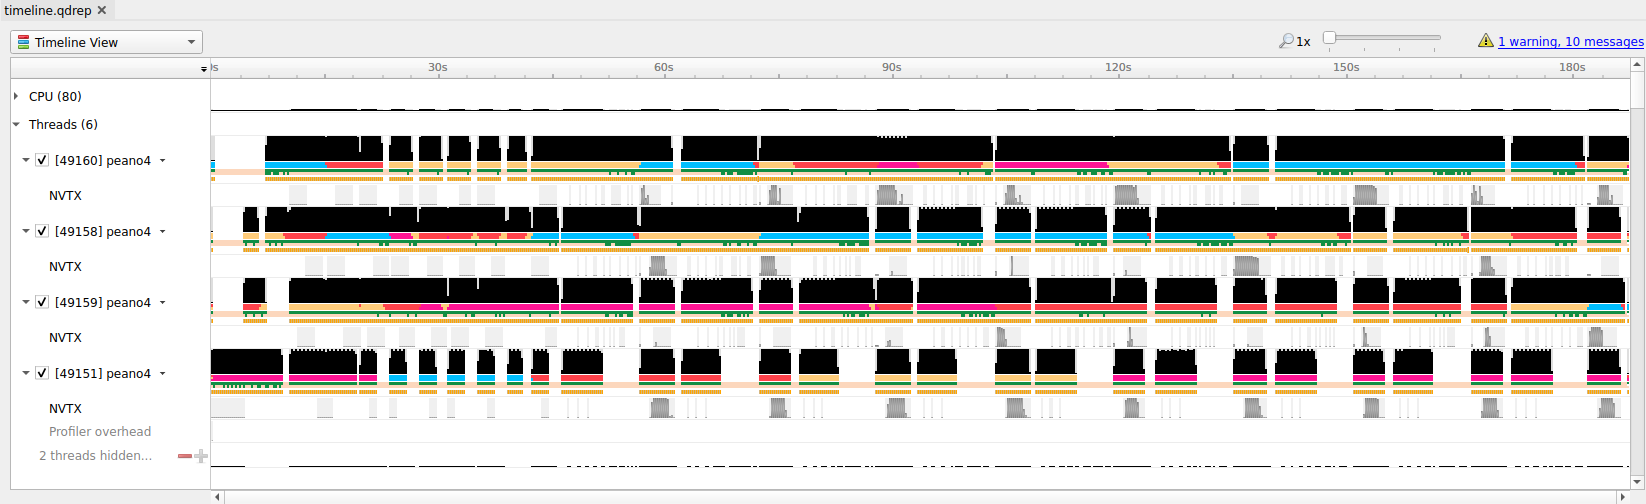
\includegraphics[width=0.9\textwidth]{21_task-priorities/nsight.png}
\end{center}

\noindent
The above illustration is an illustration with NVIDIA Nsight Systems 2020.3.1.
The code did nine time steps, and each time step consists of two grid sweeps. 
We see this pattern clearly in the last thread. 
We also see that this decomposition is ill-balanced, as two threads are very
busy all the time, one is reasonably busy, and one faces quite some idle time.
This setup is ill-balanced and the task distribution does not work as it should
be.

\begin{center}
 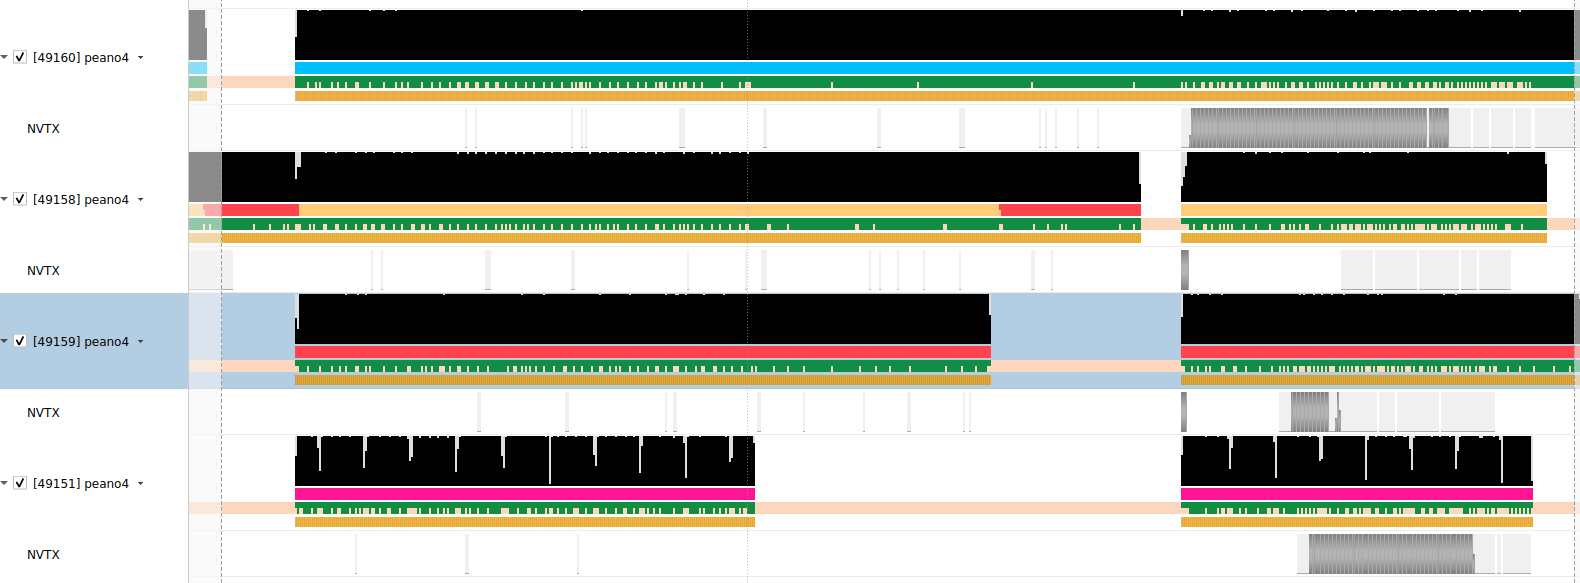
\includegraphics[width=0.9\textwidth]{21_task-priorities/zoom-in.png}
\end{center}


\noindent
A zoom-in (remember that two blackish bars above represent one time step)
reveals that the majority of enclave tasks is handled on the first thread which
is the slowest ones.
These are the dark grey bars in the illustration below.



\subsection{What we should see}

\Peano\ splits up each time step into two mesh traversals.
Each mesh traversal runs through one of the (four) subdomains as introduced
above. 
The first traversal runs through the mesh and issues a lot of tasks.
It also solves some Finite Volume problems and issues the MPI messages (not
relevant here).
The tasks should go into the background, as they are low priority (background
tasks).
This first traversal is ill-balanced, as the mesh decomposition is slightly
ill-balanced.


In the second traversal, each thread runs again through its domain.
This time, it waits per cell for which we have issued a background task before
until its task is done.
Throughout this wait, it processes some of the tasks.
The traversals per se again are ill-balanced. 


What we should see is that three out of four traversals needs pretty much the
same time, as the grid is decomposed into three big chunks plus one smaller one.
We should also see that the background tasks (dark items) slot into the idle
time of the briefer task.


\subsection{Data flow spec}

The underlying code is realised as follows (this is a generic pattern that I
use for all implementation backends):

\begin{enumerate}
  \item The code runs through the domain parts with a big parallel for.
  \item The parallel fors spawn background tasks. They can either be real tasks
  (with low priority) or we enqueue them manually into a task container.
  \item The code issues tells the task system once that it has finished its
  traversal (see below).
  \item The code runs through the domain parts once more with a big parallel
  for.
  \item Per cell, it checks whether it has spawned a task before and whether
  this task outcome is already there.
  \item If the task is not there, the traversal processes one task from the
  background queue (it could also yield) and checks again, i.e.~the checks
  realise (logically) some kind of busy polling.
\end{enumerate}


\subsection{Code regions causing the behaviour}

All code that leads to the discussed behaviour can be found in
\texttt{src/tarch/multicore/tbb/Tasks.cpp} or
\texttt{src/tarch/multicore/omp/Tasks.cpp}, respectively.
The routine that is responsible for the parallel mesh run-through (grid
traversals) is called \texttt{tarch::multicore::spawnAndWait()}.


The handling of the parallel tasks is done in
\texttt{tarch::multicore::processPendingTasks()} which each traversal calls
\begin{itemize}
  \item once after it has finished its local traversal (with the parameter 0 to
  indicate that it is not waiting for anything but it might be a good idea go
  launch some task progression threads);
  \item every time the code waits for a background task outcome (with the
  parameter 1, as it says ``do one task and return so I can check whether the
  result I'm waiting for meanwhile has dropped in'').
\end{itemize}


\section{Flaws identified}


\subsection{OpenMP: task group}

I have used a simple OpenMP task group
\begin{code}
void tarch::multicore::spawnAndWait(
  const std::vector< Task* >&  tasks
) {
  #pragma omp taskgroup
  for (int i=1; i<tasks.size(); i++) {
    #pragma omp task
    {
      bool reschedule = tasks[i]->run();
      assertion( not reschedule ); // these tasks should run only once
      delete tasks[i];
    }
  }
}
\end{code}

\noindent
It seems that this snippet uses five threads for four subpartitions,
i.e.~creates a task tree of height one where the parent task of the newly
created tasks does some busy waiting.
This is unfortunate, as further tasks might remain in the system which
should/could be processed meanwhile (see next item).



\subsection{OpenMP: task group}

If I use a task group, it seems that no further OpenMP tasks are progressed
while I wait for all child tasks to terminate.
Idle time is thus not used efficiently.
The tasks in \Peano\ can last for quite a while (they are whole domain
traversals), i.e.~kicking one thread out of the system through busy
polling/active waiting is kind of a waste.
Therefore, we need a more elegant solution here.
